\section{Background}

\subsection{Tensorcontractions}
\label{Tensorcontractions}

%TODO: HOW THE HELL DO I INTRODUCE MATH?!
Tensorcontractions are a generalization from batched matrix multiplications on n-dimensional Arrays called order-n tensors.
Imagine contraction of an order-$n$ tensor $A \in \mathbb{R}^{I_1\times\dots\times I_n}$ and an order-$m$ tensor $B \in \mathbb{R}^{J_1\times\dots\times J_m}$ with k shared dimensions to multiply to a new order-$(n+m-k)$ tensor $C \in \mathbb{R}^{K^1\times\dots\times K^{(n+m-k)}}$.
As an example from "Einsum is all you need" \cite{einsum_is_all_you_need} imagine $n=4, m=5$, $I_2 = J_3$ and $I_3 = J_5$.
The resulting Tensor $C$ would be computed as $C_{pstuv}=\sum_{q}\sum_{r}A_{pqrs}B_{tuqvr}$.

\subsection{Einsum expressions}

Einsumexpressions allow for a more succinct expression than the typical Tensor notation as used in \ref{Tensorcontractions}.
Instead of writing $C_{pstuv}=\sum_{q}\sum_{r}A_{pqrs}B_{tuqvr}$ the same contraction is expressed as $A_{pqrs}B_{tuqvr} \rightarrow C_{pstuv}$.
The summation signs are now implicit.
Einsumexpressions can also describe the contractions from more than 2 tensors\cite{einsum_is_all_you_need}.
Instead of writing $D_{ij} = \sum_{k}\sum_{l}A_{ik}B_{jkl}C_{il}$ it is expressed as $A_{ik}B_{jkl}C_{il} \rightarrow D_{ij}$.
The evaluation of einsum expression is supported in the popular frameworks Torch\cite{torch}, PyTorch\cite{pytorch} and Tensorflow\cite{tensorflow}.

\subsection{einsum\_ir}

\begin{figure}[ht]
  \centering{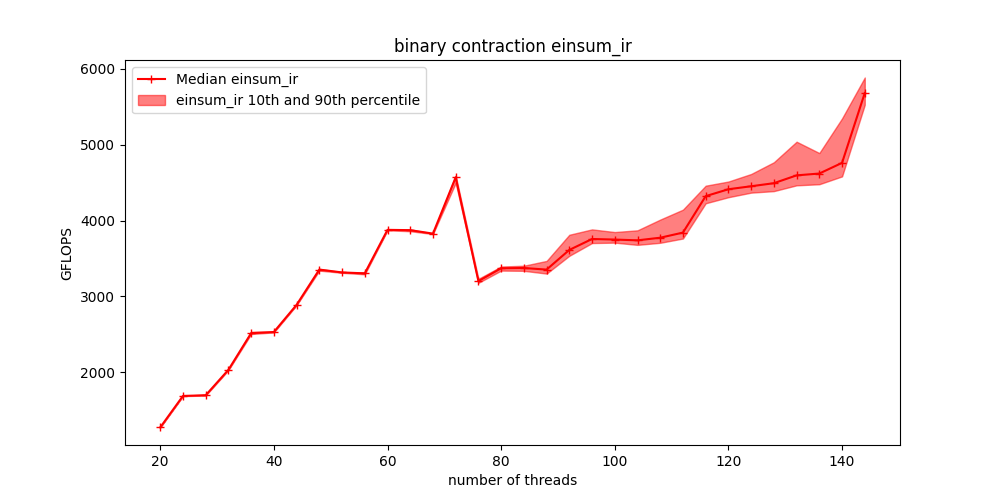
\includegraphics[width=0.95\textwidth]{gflops_threads.png}}
  \caption{
    Performance of existing einsum\_ir on an Nvidia Grace CPU superchip.
    Grace consists of 2 72-core cpus connected with NVLink.
  }
  \label{fig:perf_threads}
\end{figure}

\texttt{einsum\_ir}\cite{einsum_ir} is a software library developed at the Friedrich Schiller University Jena to accelerate a series of einsum expressions in C++.
It takes an einsum tree as input and evaluates its root recursively.
My work will build on top of the existing work done in this library.
Specifically I will use their implementation of a binary tensor contraction $A,B \rightarrow C$ as local primitive for my algorithm.
\texttt{einsum\_ir} already implements shared memory parallelisation with OpenMP\cite{openMP}, so it can already exploit all cpu cores on a single NUMA domain.
Its performance is currently not scaling well across more than one cpu, as seen in Figure \ref{fig:perf_threads}.
The performance drops as soon as the threads of the second cpu get used, as seen in the sharp decline after 72 threads.
This thesis provides algorithms aimed at a secondary distributed memory parallelization to alleviate that issue.
An important note for the current binary tensor contraction interface is that it expects all tensors, both input and output, to be contiguous in memory.
